\documentclass[11pt]{article}
\usepackage{amsmath}
%\usepackage{extsizes}
\usepackage{amsmath,amssymb}
%\usepackage{omegavn,ocmrvn}
%\usepackage[utf8x]{inputenc}
\usepackage[utf8]{vietnam}

\usepackage{listings}
\lstset{language=Python}          % Set your language (you can change the language for each code-block optionally)


\usepackage{longtable}
\usepackage{answers}
\usepackage{graphicx}
\usepackage{array}
\usepackage{pifont}
\usepackage{picinpar}
\usepackage{enumerate}
\usepackage[top=3.0cm, bottom=3.5cm, left=3.5cm, right=2.5cm] {geometry}
\usepackage{hyperref}


\newtheorem{bt}{Câu}
\newcommand{\RR}{\mathbb R}
\Newassociation{sol}{Solution}{ans}
\newtheorem{ex}{Câu}
\renewcommand{\solutionstyle}[1]{\textbf{ #1}.}


\begin{document}
% \noindent
\begin{tabular*}
{\linewidth}{c>{\centering\hspace{0pt}} p{.7\textwidth}}
Trường ĐHKHTN, ĐHQGHN & {\bf Học Kỳ 1 (2019-2020)}
\tabularnewline
K62 TTƯD & {\bf Bài Tập Giải Tích Số. No 11 \\ IVP - 5 phương pháp ẩn/hiện cơ bản}
\tabularnewline
\rule{1in}{1pt}  \small  & \rule{2in}{1pt} %(Due date:)
\tabularnewline

%  \tabularnewline
%  &(Đề thi có 1 trang)
\end{tabular*}
%
% \Opensolutionfile{ans}[ans1]

\begin{bt}
a) Chứng minh rằng hàm số $y(t) = t^2/4$ là lời giải của bài toán giá trị ban đầu
\begin{equation*}
y'(t) = \sqrt{y} \quad ; \  y(0) = 0. 
\end{equation*}
b) Hãy thực hiện hai bước với bước $h = 0.2$ bằng cả 3 công thức hiện và 2 công thức ẩn. \\
c) Viết script trong Python áp dụng cả 2 phương pháp Euler ẩn và hiện với bước đi $h = 0.01$ để xác định nghiệm số. Vẽ đồ thị và so sánh sai số tuyệt đối của hai phương pháp Euler trên. \\
d) Viết script trong Python áp dụng các phương pháp hình thang ẩn, hiện, trung điểm hiện với bước đi $h = 0.01$ để xác định nghiệm số. Vẽ đồ thị và so sánh sai số tuyệt đối của 3 sai số của các phương pháp trên.
\end{bt}

\begin{bt}
Cùng câu hỏi với bài tập 1 cho bài toán giá trị ban đầu
\begin{equation*}
y'(t) = - 4y + t^2  \ \mbox{ với } \ t\in [0,1] \quad ; \  y(0) = 1. 
\end{equation*}
a) Hãy thực hiện hai bước với bước $h = 0.2$ bằng cả 3 công thức hiện và 2 công thức ẩn. \\
b) Viết script trong Python áp dụng cả 5 phương pháp trên với bước đi $h = 0.01$ để xác định nghiệm số. Vẽ đồ thị và so sánh sai số tuyệt đối của 5 phương pháp trên.
Cho nghiệm chính xác là 
%
\[
y = \dfrac{31}{32} e^{-4x} + \dfrac{1}{4} x^2 - \dfrac{1}{8} x + \dfrac{1}{32}
\]
%
\end{bt}

\begin{bt} Viết các hàm trong Python để tính tích phân dựa trên 5 phương pháp ẩn và hiện cơ sở, ví dụ 
%
\begin{lstlisting}[frame=single] 
def Euler_hien(f,t0,tf,h):
return y , t
\end{lstlisting}
%	 
trong đó $f = f(t,y)$ là hàm \quad ; $t \in [t0,tf]$ là khoảng thời gian, $h$ là độ rộng mỗi bước và được cho trước. Chú ý các nút được sử dụng là cách đều, tức là $t_0<t_1<\dots<t_f$, $t_i = a+i*h$, $h=\cfrac{tf-t0}{n}$. 


\end{bt}

\centerline{———————————Hết——————————-}

\centering{------------------------------Phần 4: Các phương pháp lặp --------------------------------------}

\begin{center}
	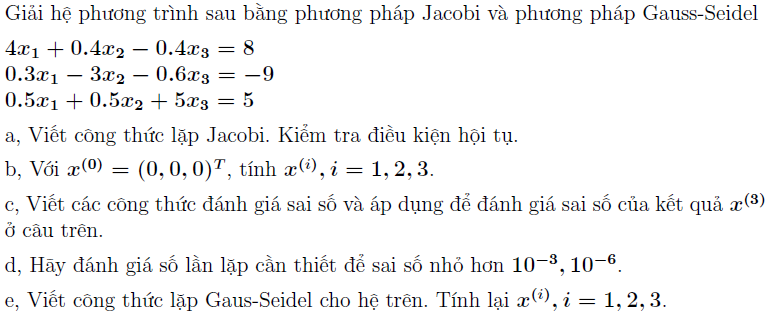
\includegraphics[scale = 0.7]{4}	
\end{center}

\begin{bt}
\end{bt}
\begin{figure}[H]
	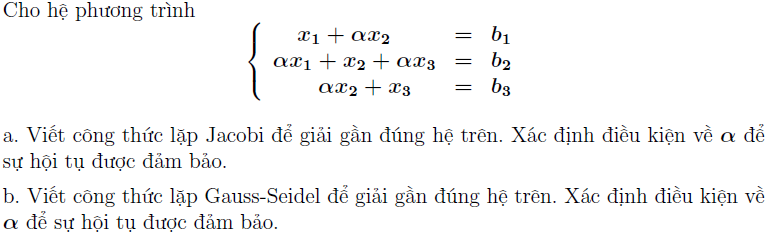
\includegraphics[scale = 0.7]{5}
\end{figure}
c. Từ các tính toán ở hai câu trên, hãy so sánh tốc độ hội tụ của hai phương pháp.


\end{document}

\vspace{1cm}
\noindent{\bf Chú ý:} {\it Cán bộ coi thi không giải thích gì thêm}\\
\Closesolutionfile{ans}
\newpage
\begin{center}
{\LARGE{\bf ĐÁP ÁN}}
\end{center}

\begin{sol}
	\begin{figure}[h!]
		\centering
		\includegraphics[width=0.8\linewidth]{Solution1/Sol4_1.png}
		%\caption{}
		\label{fig:Sol4}
	\end{figure}
	Exercise 7: Convergence order is 3.	
\end{sol}

   
\end{document}



